\documentclass[letterpaper, 12 pt, conference]{ieeeconf}

\IEEEoverridecommandlockouts
% This command is only needed if 
% you want to use the \thanks command

\overrideIEEEmargins
% Needed to meet printer requirements.
%\usepackage[margin=0.65in]{geometry}

% See the \addtolength command later in the file to balance the column lengths
% on the last page of the document

% The following packages can be found on http:\\www.ctan.org
\usepackage{graphics} % for pdf, bitmapped graphics files
\usepackage{epsfig} % for postscript graphics files
\usepackage{mathptmx} % assumes new font selection scheme installed
\usepackage{times} % assumes new font selection scheme installed
\usepackage{amsmath} % assumes amsmath package installed
\usepackage{amssymb}  % assumes amsmath package installed

\usepackage{hyperref}
\usepackage{url}
%\usepackage[pdftex]{graphicx}
%\usepackage{amsfonts}
\usepackage{subfigure} 
\usepackage{algorithm}
%\usepackage{algorithmic}
\usepackage{algcompatible}
\usepackage{framed}
\usepackage{balance}
\graphicspath{{images/}}

\title{\LARGE \bf
Generating Natural Language Descriptions of Trajectories Using Long Short Term Memory Neural Networks}

\author{Rodolfo Corona and Rolando Fernandez}

\begin{document}

\maketitle
\thispagestyle{empty}
\pagestyle{empty}

\section{Problem Description}

Given a point-cloud $p$ $\in$ $P$ and a manipulation trajectory $t$ $\in$ $T$, our goal is to output a free-form  Natural Language (NL) description $l$ $\in$ $L$ that describes the trajectory $t$:

\begin{equation}
f: T\times P \mapsto L
\end{equation}

\section{Methods}

\subsection{Robobarista Dataset}

Sung et al. developed the Robobarista framework in order perform Deep Multimodal embedding of Point Clouds and NL Descriptions to Trajectories, as shown in Equation (2). Sung et al. aimed to create a system for manipulation planning which could generalize to different objects with similar parts to be manipulated \cite{sung2016robobarista}. 

\begin{equation}
f: P\times L \mapsto T
\end{equation}

Using the Robobarista framework Sung et al. collected an extensive dataset of consisting of triplets of the form (Point Cloud, NL Descriptions, and Trajectory). The dataset consists of 116 objects with 249 parts along with 250 NL instructions, for which there was collected 1225 manipulation trajectories. 

Each of the 116 objects is split into parts depending on the number of NL instructions that pertain to it and the original point cloud scene is segmented with respect to the part frames, being stored as a Comma Separated Value (CSV) file consisting of [x,y,z,r,g,b] values. 

Furthermore, each of the objects have multiple manipulation trajectories for each part stored as a list of waypoints \cite{sung2016robobarista}. For our experiments we split the dataset into 5 folds of train and test data in order to perform 5 fold cross validation at the end of our experiments.

\subsection{Baseline with Point Clouds}
For our initial baseline we created a pipeline that utilizes the Point Clouds and NL descriptions in the Robobarista dataset to perform inference using K-Means clustering and K-Nearest Neighbors (Figure \ref{fig:Baseline_Point_Cloud}). We first train a K-Means model and a KNN model using the training data for each of the 5 folds.

The Point Cloud key points are taken from the segmented object part point cloud CSV files. We create two vectors from the CSV files, one is a vector of all the Point Clouds in the training set where the Point Clouds themselves are vectors of key points and the other is a vector of all the key points in the training set. 

Utilizing the K-Means algorithm in the Python SKLearn package, we input the vector of all the key points in the training set into the K-Means algorithm with a cluster count of 50 and get back trained K-Means model. With the K-Means model we extract a closest cluster prediction for the key points in each individual Point Cloud in the vector of all the Point Clouds in the training set. Then using the cluster predictions we compute a bag of features (BOF) vector for each Point Cloud based on the number of occurrences of each cluster.

The BOF vectors are then used as input with a neighbor count of 1 to the K-Nearest Neighbors classifier in the Python SKLearn package and in return we get a trained KNN model. We are then able to use this KNN model to determine the nearest neighbors of a given Point Cloud. 


\begin{figure}[htb!]
  \centering
  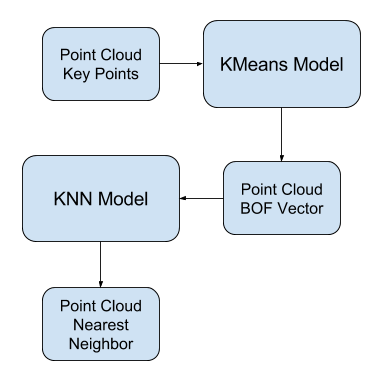
\includegraphics[width=0.3\textwidth]{Baseline-[Point_Cloud]}
  \caption{Baseline with Point Clouds}
  \label{fig:Baseline_Point_Cloud}
\end{figure}

\subsection{LSTM Implementation}

\section{Results}

\subsection{Baseline with Point Clouds}

For the baseline we conducted experiments using the data from each of the 5 folds, running a total of 5 trials. For each trial we created a gold reference consisting of the already known NL descriptions for each of the point clouds and a test reference consisting of the NL description returned by using the trained K-Means and KNN models.

Each point cloud in the fold test data is first inputed in the K-Means model to extract the BOF vector representation, then the BOF vector is inputed into the KNN model to retrieve the nearest neighbor of the point cloud, and lastly we look up the NL description for the given neighbor. With the completed the test and gold reference files we are then able to use the sentence comparison package METEOR to evaluate the accuracy of the Baseline with Point Clouds .

On average the baseline performed poorly as only reaching its highest performance in the first fold achieving a final Meteor score of 0.172. These results were expected as the Baseline only performs a simple lookup based on nearest neighbor inference and is not able to adapt properly.

\begin{figure}[htb!]
  \centering
  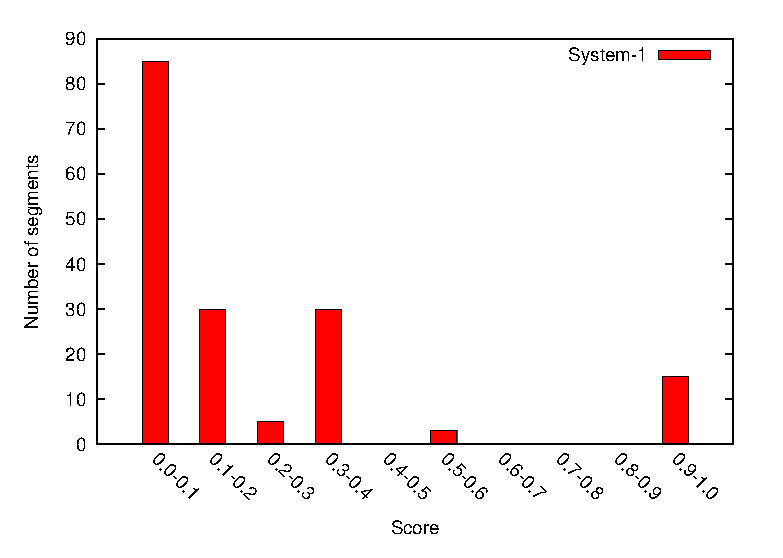
\includegraphics[width=0.45\textwidth]{fold_1_score}
  \caption{Meteor Score for Fold 1 Test Data}
  \label{fig:fold_1_score}
\end{figure}

\begin{figure}[htb!]
  \centering
  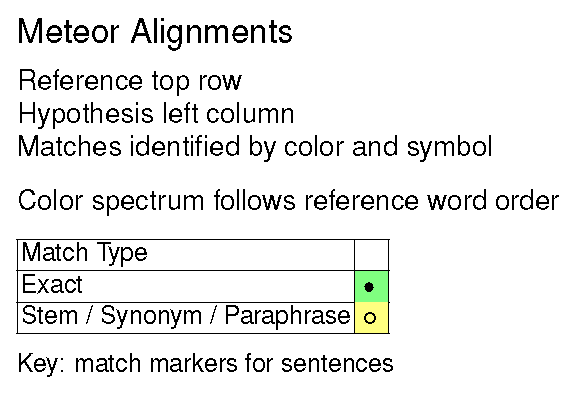
\includegraphics[width=0.45\textwidth]{meteor_alignment_key}
  \caption{Meteor Alignment Key}
  \label{fig:meteor_alignment_key}
\end{figure}

\begin{figure}[htb!]
  \centering
  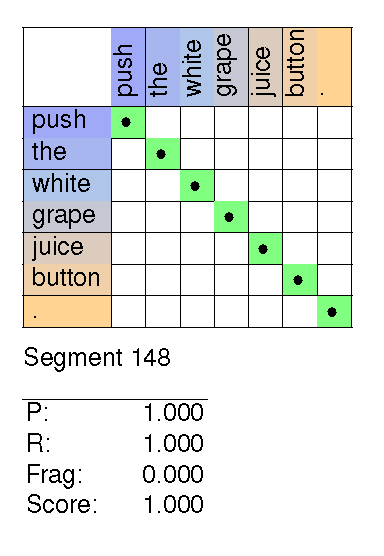
\includegraphics[width=0.3\textwidth]{fold_1_sentence_148}
  \caption{Meteor Alignment for Fold 1 Sentence 148}
  \label{fig:fold_1_sentence_148}
\end{figure}

\begin{figure}[htb!]
  \centering
  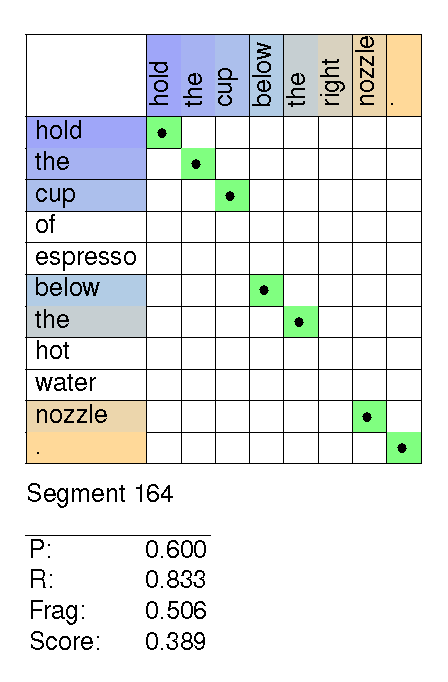
\includegraphics[width=0.3\textwidth]{fold_1_sentence_164}
  \caption{Meteor Alignment for Fold 1 Sentence 164}
  \label{fig:fold_1_sentence_164}
\end{figure}

\subsection{LSTM Implementation}

\section{Outlook}

\section{Future Work}

\section{Justification of Progress}


%\bibliographystyle{abbrv}
\bibliographystyle{IEEEtran}
\bibliography{citations}

\end{document}
